\chapter{Compression of probability distributions}
\label{ch:pdf_compression}


\begin{chapabstract}
  The entropy bottleneck introduced by Ballé~\emph{et~al.}~\cite{balle2018variational} is a common component used in many learned compression models.
  It encodes a transformed latent representation using a static distribution whose parameters are learned during training.
  However, the actual distribution of the latent data may vary wildly across different inputs.
  The static distribution attempts to encompass all possible input distributions, thus fitting none of them particularly well.
  This unfortunate phenomenon, sometimes known as the amortization gap, results in suboptimal compression rates.
  Moreover, the transform also suffers difficulties from being constrained into targeting an inflexible static distribution, leading to further inefficiencies.
  To address these issues, we propose a method that dynamically adapts the encoding distribution to match the latent data distribution for a specific input.
  First, our model estimates a better encoding distribution for a given input.
  This distribution is then compressed and transmitted as an additional side-information bitstream.
  Finally, the decoder reconstructs the encoding distribution and uses it to decompress the corresponding latent data.
  Our method achieves a BD-rate gain of -6.95\% on the Kodak test dataset when applied to the standard fully factorized architecture.
  % When used in conjunction with a parallelized RDOQ strategy, the BD-rate shows a gain of TODO\%.
  Furthermore, the transform used by our method costs only as few as 10 MACs/pixel, in contrast to related side-information methods such as the scale hyperprior, which costs at least 1300 MACs/pixel.
\end{chapabstract}




% TODO(review): Rephrase more compactly.
\section{Introduction}
\label{sec:pdf_compression/intro}

At the heart of compression is the probability distribution.
% We have an input distribution (usually, abstract, and undefinable).
% A dataset is a sampling of that distribution.
Typically, we model the data to be compressed using a probability distribution.
It is less common to model the probability distribution itself.
Nonetheless, as will soon see, there is potential value in doing so.

In this chapter, we explore the compression of probability distributions that are used in compression.
Specifically, we will focus on probability distributions that are used to model the latent representations produced by an image compression model.
The entropy models of learned image compression models utilize probability distributions to compress transformed latent representations.
For example, Ballé~\emph{et~al.}~\cite{balle2018variational} model a latent representation $\boldvar{y}$ using the following entropy models:
\begin{enumerate}
  \item
    A "fully factorized" \emph{entropy bottleneck}.
    Each element ${y}_{c,i}$ within the $c$-th channel is modelled using a single channel-specific non-parametric probability distribution ${p}_{c}(y)$, which is fixed once training completes.
    That is, the elements ${y}_{c,1}, {y}_{c,2}, \ldots, {y}_{c,H W}$ within the $c$-th channel are assumed to be drawn from independent and identically distributed (i.i.d.) random variables with the probability distribution ${p}_c(y)$.
  \item
    A \emph{Gaussian conditional}.
    For each element ${y}_{i}$, the parameters ${\mu}_{i}$ and ${\sigma}_{i}$ of its encoding distribution are computed, conditioned on the latent representation $\boldvar{z} = h_a(\boldvar{y})$.
    In some cases, the modeling distribution is a mixture of $K$ Gaussians --- known as a Gaussian mixture model (GMM) --- with parameters ${\mu}_{i}^{(k)}$ and ${\sigma}_{i}^{(k)}$ for each Gaussian, alongside an affine combination of weights ${w}_{i}^{(K)}$ that satisfy the constraint $\sum_k {w}_{i}^{(k)} = 1$.
\end{enumerate}
Both of these have their advantages and disadvantages.
Of these two, the entropy bottleneck is the most flexible at modeling arbitrary distributions.
Indeed, it often does, modeling many channels via Laplacian-like distributions, which the latent representations often tend towards.
However, because all elements within a given channel are modelled using the same distribution, it is quite poor at specializing and adapting to specific input distributions.
Instead, it models a "conservative" distribution that tries to encompass all possible inputs, which is often suboptimal, as we will show later in this chapter.
This is sometimes known as the \emph{amortization gap}~\cite{balcilar2022amortizationgap,cremer2018inferencesuboptimality}.
In contrast, the Gaussian conditional is better at adapting to a specific input, though it is limited to modeling Gaussian distributions.
Furthermore, it must also pay an additional cost for transmitting the distribution parameters, though this is often worth the trade-off, e.g., a savings of roughly 40\% for a 10\% increase in rate, as shown by~\cite{balle2018variational}.

In their "scale hyperprior" architecture, Ballé~\emph{et~al.}~\cite{balle2018variational} utilize an entropy bottleneck to compress the latent representation $\boldvar{z} = h_a(\boldvar{y})$.
This is known as "side-information", and its compressed bitstream is transmitted before the bitstream for $\boldvar{y}$.
The reconstructed latent $\boldvar{\hat{z}}$ is then used to determine the parameters%
\footnote{In their initial publication, $\boldvar{\mu}$ is fixed to $0$, though later results~\cite{minnen2018joint} show that it is better to predict $\boldvar{\mu}$ as well.}
$\boldvar{\mu}$ and $\boldvar{\sigma}$ of a Gaussian conditional distribution which is used to reconstruct $\boldvar{\hat{y}}$.
More sophisticated entropy models, such as ELIC~\cite{he2022elic} use multiple successive applications of the Gaussian conditional entropy model, alongside an entropy bottleneck functioning as a "scale hyperprior".
In many such models that utilize the scale hyperprior, the rate usage of the entropy bottleneck often comprises roughly 10\% of the total rate.
Evidently, the entropy bottleneck is a key component of many state-of-the-art (SOTA) image compression models, and so it is important to address the amortization gap suffered by the entropy bottleneck.

In this chapter, we propose a method to address this amortization gap via the compression of an input-specific probability distribution. % input-adaptive?
This allows the entropy bottleneck method to adapt to the input distribution, rather than using a fixed dataset-optimized probability distribution which suffers from the amortization gap.
We demonstrate that our input-adaptive method can be used by models containing the entropy bottleneck in order to achieve better rate-distortion performance.




\section{Related works}
\label{sec:pdf_compression/related}

In Campos~\emph{et~al.}~\cite{campos2019content}, the latent $y$ is refined by performing gradient descent to optimize it, while holding the trained model parameters fixed.
This is effectively a form of Rate-Distortion Optimized Quantization (RDOQ), though the optimized loss
$L = R_{\boldvar{\tilde{y}}} + \lambda_x D(\boldvar{x}, \boldvar{\tilde{x}})$
is not precisely aware of the exact effect of quantization.  % TODO(review): reword?

Balcilar~\emph{et~al.}~\cite{balcilar2022amortizationgap} propose non-learned methods for the compression and transmission of the encoding distributions.
For the factorized entropy model, they first measure a discrete histogram of the $c$-th latent channel.
Then, they construct an approximation of the histogram using a $K$-Gaussian mixture model parameterized by $w^{(k)}$, $\mu^{(k)}$, and $\sigma^{(k)}$.
The aforementioned parameters are compactly encoded into 8~bits each, and transmitted.
That is, for a model using $C$ activated channels, $(3K - 1) \cdot C \cdot 8$ bits are required to transmit the parameters.
(Typically, $K \in [1, 3]$ is used, and $C \in [16, 192]$ for low-rate models.)
The approximation model is then used as the encoding distribution
$p_{\boldvar{\hat{y}}}(\boldvar{\hat{y}}_c) = \sum_{k=1}^K w_k \; \mathcal{\hat{N}}(\boldvar{\hat{y}}_c ; \, \mu_k, \, {\sigma_k}^2)$.
For the Gaussian conditional entropy model, they instead transmit a factor $\beta^{(c)}$ that corrects the error in the center (and most likely) bin's probability.
A key difference between our work and this prior work is that we formulate a learnable method for the compression of the encoding distribution.

Galpin~\emph{et~al.}~\cite{galpin2023entropy} introduce a lightweight non-learned context model for raster-scan ordered encoding, similar to Minnen~\emph{et~al.}~\cite{minnen2018joint}.
They also implement a simple raster-scan ordered greedy RDOQ method which repeatedly reruns the decoder on the quantized y hat to discretely optimize the loss.
To reduce the computational cost of the RDOQ process, the loss estimation is restricted within the receptive field (a $9 \times 9$ latent window) and only delta y hat in $\{-1, 0, +1\}$ is explored.
They then compare their proposed methods in conjunction with~\cite{campos2019content,balcilar2022amortizationgap} in various configurations on both the standard factorized model and its GDN to ReLU replacement model variant.

% Orange Labs - "COOL-CHIC: Coordinate-based Low Complexity Hierarchical Image Codec"
% https://arxiv.org/abs/2212.05458
%
% Orange Labs - "Low-complexity Overfitted Neural Image Codec"
% https://arxiv.org/abs/2307.12706




\section{Proposed method}

\subsection{Compression of probability distributions}

% Clarify, collection of probability distributions?
% $\boldvar{p} = (\boldvar{p}_1, \boldvar{p}_2, \ldots, \boldvar{p}_M)$ is a collection of probability distributions, one for each channel.

Let $\boldvar{x}$ be an input image, and $\boldvar{y} = g_a(\boldvar{x})$ be its transformed latent representation.
Consider a fully-factorized entropy model~\cite{balle2018variational}, which models $\boldvar{\hat{y}} = \operatorname{Quantize}[\boldvar{y}]$ using a single channel-specific non-parametric probability distribution $\boldvar{\hat{p}}_j$ for each channel $j$.
Since all elements within a given channel are modelled using the same distribution, in this setting, the "true" probability distribution $\boldvar{p}_j$ for the $j$-th channel of $\boldvar{y}$ can be determined exactly by computing the normalized histogram of $\boldvar{\hat{y}}_j$.
The true distribution for the $j$-th channel is also the encoding distribution $\hat{\boldvar{p}}_j$ with the minimum rate cost for encoding a specific latent representation $\boldvar{\hat{y}}$ using the entropy model.
That is, the ideal encoding distribution $\boldvar{\hat{p}}^*_j$ is given by
\begin{equation*}
  \boldvar{\hat{p}}^*_j = \argmin_{\boldvar{\hat{p}}_j} \left[
    H(\boldvar{p}_j) + D_{\mathrm{KL}}(\boldvar{p}_j \parallel \boldvar{\hat{p}}_j)
  \right]
  \implies \boldvar{\hat{p}}^*_j = \boldvar{p}_j.
\end{equation*}
Unfortunately, using the true distribution $\boldvar{p}$ for encoding is infeasible, since the decoder does not have access to it.
% In constrast to the VAE intractibility problem, we *do* know this particular true distribution. Of course, the problem setup is a bit different...
Instead, we propose a method that generates a reconstructed approximation $\boldvar{\hat{p}}$ that targets $\boldvar{p}$, subject to a rate trade-off.
% D(p || phat) is the "distortion" of the distribution, measured in KL divergence.
% H(q) is the rate cost. (Slightly imprecise notation.)
We discuss the specific loss function that is optimized in \cref{sec:pdf_compression/loss}.

\cref{fig:pdf/pdfs} visualizes the true ($\boldvar{p}$) and reconstructed ($\boldvar{\hat{p}}$) (via our proposed method) probability distributions for a fully-factorized entropy model.
The left column shows various input images taken from the Kodak test dataset~\cite{kodak_dataset} --- except for the "(Default)" image in the first row, which is an abstract "amortized" representation of all possible input images that may be randomly drawn from the training dataset distribution.
The middle column and right columns visualize the negative log-likelihoods of the true and reconstructed probability distributions, respectively.
Each probability distribution is visualized as a 2D color plot, where
\begin{enumerate}[label=(\roman*), noitemsep, topsep=0pt]
  \item the $x$-coordinate is the channel index $j$ of the latent $\boldvar{y}$,
  \item the $y$-coordinate is the bin index $i$ of the discretized probability distribution, and
  \item the $z$-coordinate (i.e., color intensity) is the negative log-likelihood (in bits) of $(\boldvar{p}_j)_i$ or $(\boldvar{\hat{p}}_j)_i$, clipped to the range $[0, 10]$.
\end{enumerate}
% We call this representation the "PDF signature".


% TODO(figure): Rename "default" to "amortized"? Then, s/default/amortized/g.
\begin{figure}[htbp]
  \centering
  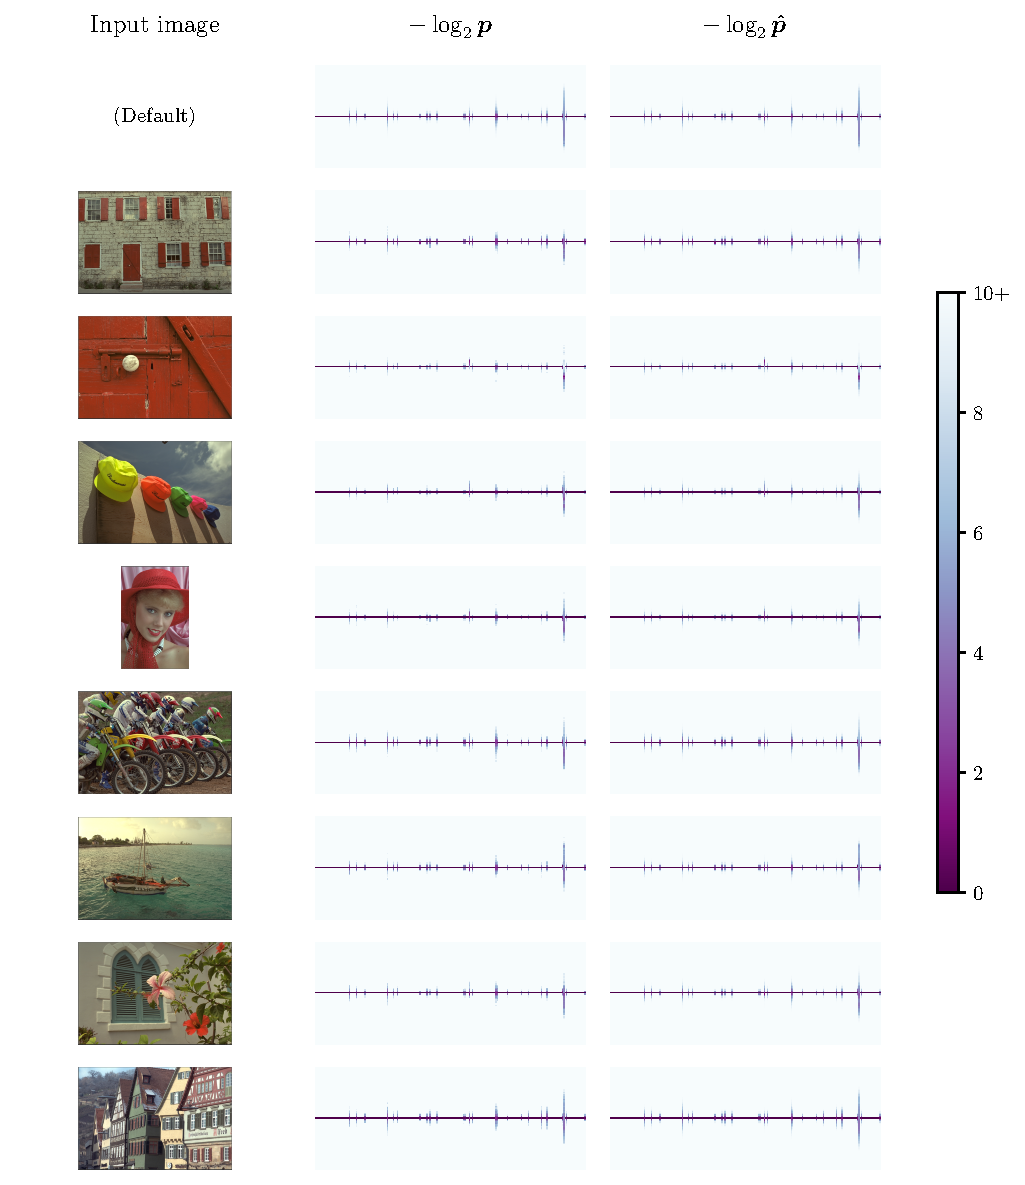
\includegraphics[width=\linewidth]{img/pdf_compression/pdfs1.pdf}
  \caption[Visualization of target and reconstructed probability distributions]{%
    Different images from the Kodak dataset, and their corresponding negative log-likelihoods (in bits) of the true and reconstructed probability distributions.%
    % TODO What quality model was used in figure?  (probably Q=3)
  }
  \label{fig:pdf/pdfs}
\end{figure}

\begin{figure}[htbp]
  \ContinuedFloat
  \centering
  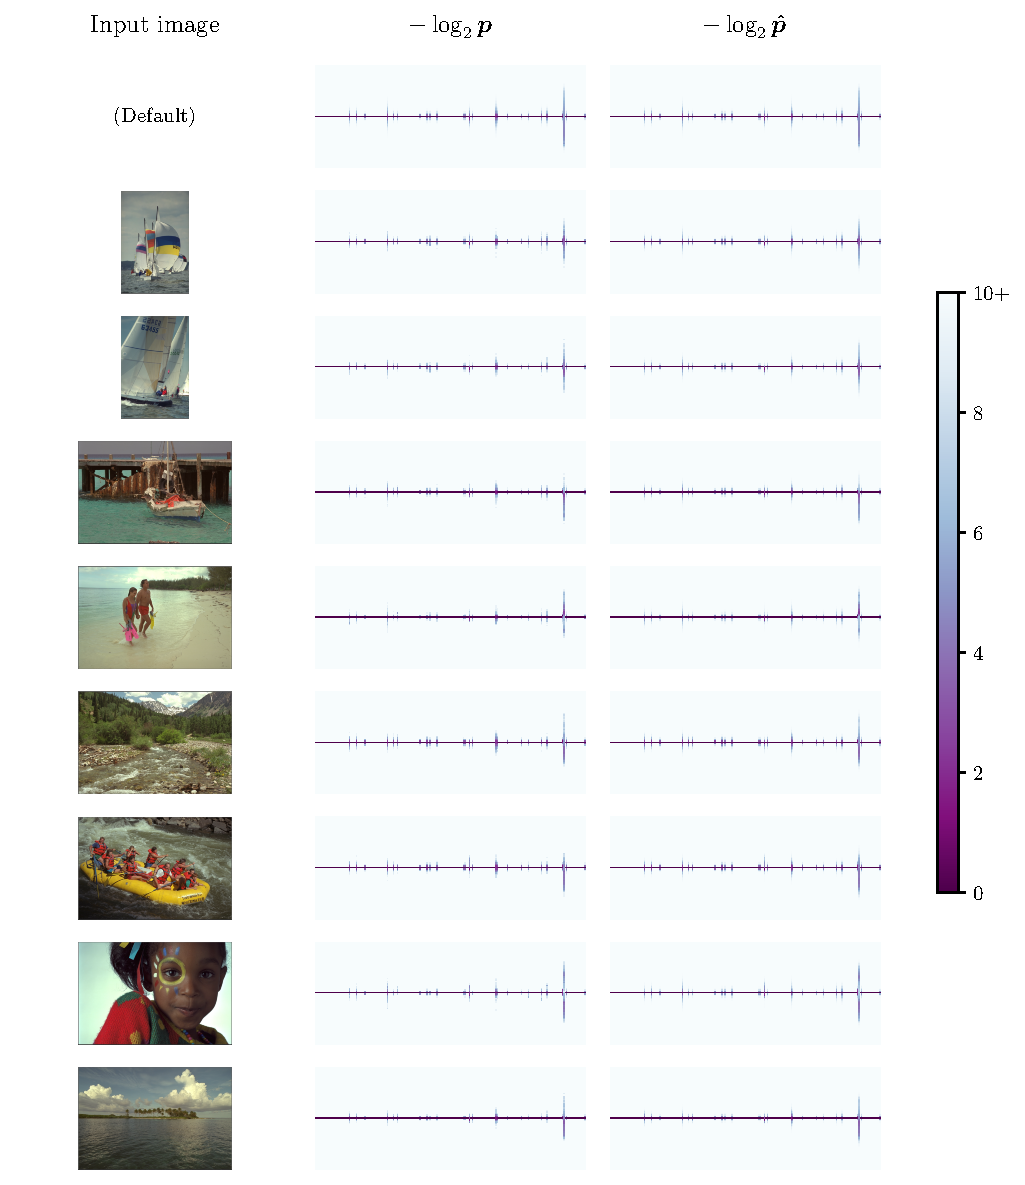
\includegraphics[width=\linewidth]{img/pdf_compression/pdfs2.pdf}
  \caption[]{(continued)}
\end{figure}

\begin{figure}[htbp]
  \ContinuedFloat
  \centering
  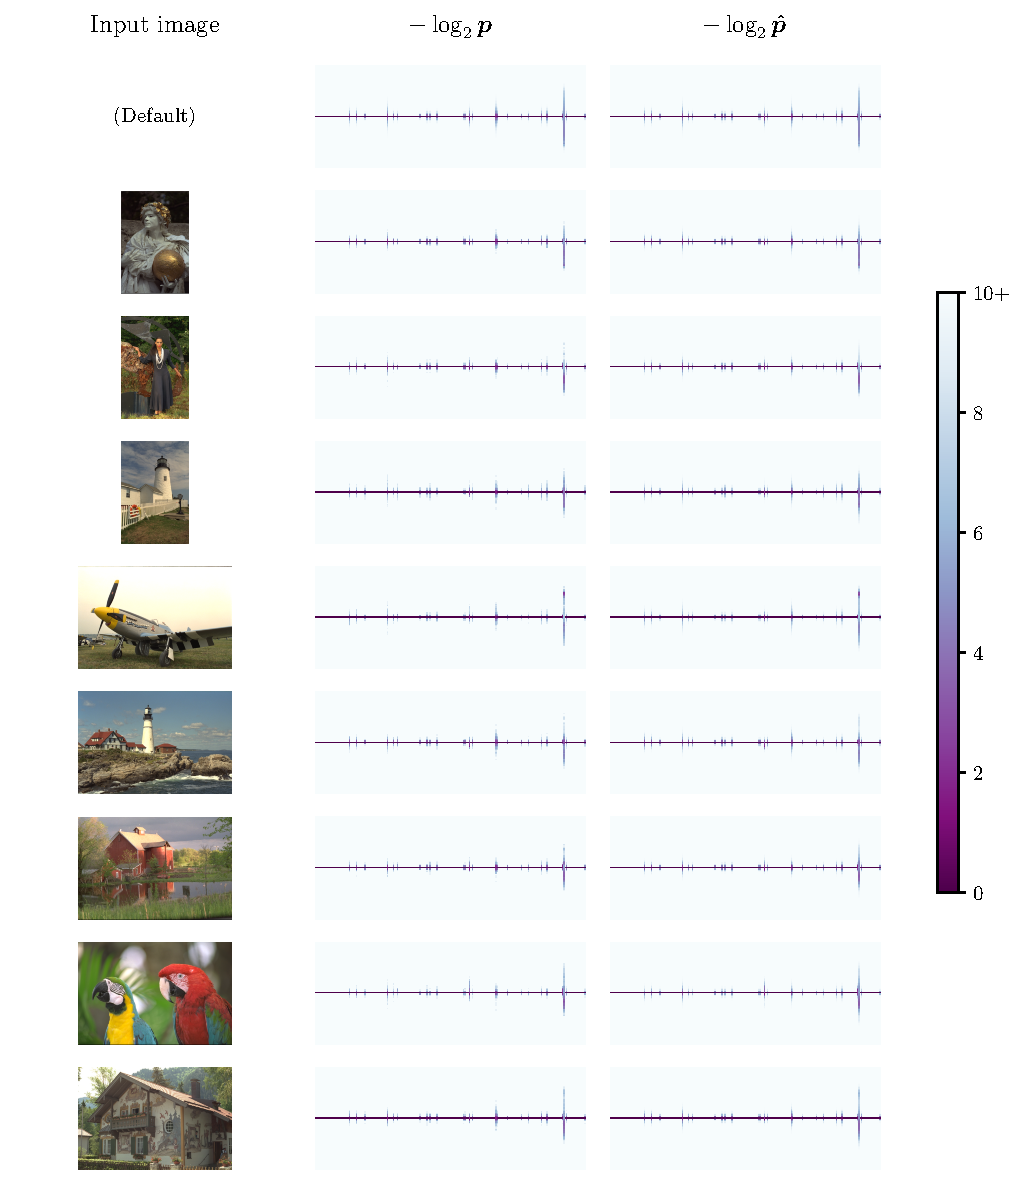
\includegraphics[width=\linewidth]{img/pdf_compression/pdfs3.pdf}
  \caption[]{(continued)}
\end{figure}

% TODO(review): Rephrase more compactly.
Evidently, the default amortized dataset-optimized probability distribution is conservative and encompasses each of the image probability distributions.
However, trying to cover all possible distributions with a single distribution leads to suboptimal compression performance since that distribution does not match each individual input distribution sufficiently well.
In contrast, with our probability distribution compression method, the encoding distribution has adapted to the probability distributions for each image.
Indeed, the true and reconstructed probability distributions look visually quite similar.
This is particularly true for high-probability regions of the true distribution, which is also where accurate reconstruction is most important.
For less probable regions, there is sometimes a larger mismatch between $\boldvar{p}$ and $\boldvar{\hat{p}}$, though this is less important, since incorrect prediction of low-probability regions has a smaller impact on the overall rate.
This indicates that our method is capable of adapting to the input distribution well, and in a way that is cognizant of the tradeoff between rates.




\subsection{Architecture overview}
\label{sec:pdf_compression/architecture_overview}

\begin{figure}[htbp]
  \centering
  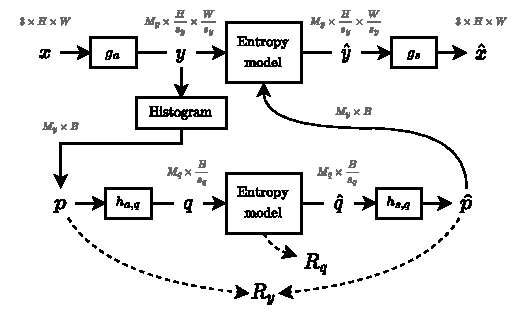
\includegraphics[width=\linewidth]{img/pdf_compression/arch-overview.pdf}
  \caption[Adaptive probability distribution compression architecture]{%
    Adaptive probability distribution compression architecture.%
  }
  \label{fig:pdf/arch}
\end{figure}

Our proposed method applied to the traditional "fully-factorized" architecture~\cite{balle2018variational} is visualized in \cref{fig:pdf/arch}.
In this configuration, the latent representation $\boldvar{y}$ is first passed through the histogram layer described in \cref{sec:pdf_compression/histogram}, which estimates the target distribution $\boldvar{p}$.
Then, $\boldvar{p}$ is passed through a distribution compression architecture consisting of the analysis transform $h_{a,q}$ which generates
a latent representation $\boldvar{q}$, followed by an entropy model (e.g. entropy bottleneck), and then finally a synthesis transform $h_{s,q}$ which reconstructs the distribution $\boldvar{\hat{p}}$.
The rate cost of encoding $\boldvar{q}$ is labelled $R_{q}$, and the rate cost of encoding $\boldvar{y}$ using $\boldvar{\hat{p}}$ is labelled $R_{y}$.




\subsection{Histogram estimation}
\label{sec:pdf_compression/histogram}

In the entropy bottleneck, the probability distribution for a given channel is fixed, regardless of the input.
In order to adapt this distribution to the input, we must first estimate the input distribution more accurately.
We do so by estimating the input distribution using a histogram.
In order to ensure differentiability backwards through the histogram module, we use the method of kernel density estimation (KDE).

% NOTE: We use p_ji and p_i too...

Let $[y_{\mathrm{min}}, y_{\mathrm{max}}]$ be a supporting domain that encompasses all values $y_1, y_2, \ldots, y_{N}$ in a specific channel.
Let $\{b_1, b_2, \ldots, b_B\}$ denote the bin centers of the $B$-bin histogram, where $b_i = y_{\mathrm{min}} + i - 1$.
In the method of kernel density estimation, which is used to estimate the probability density function from a set of observations, a kernel function is placed centered at each observed sample, and those functions are summed to create the overall density function.
To construct the histogram, we evaluate the kernel density estimate at each $b_i$.
Or rather, we use an equivalent formulation where we instead place a kernel function at each bin center, as visualized in \cref{fig:pdf/kernels}.
Then, the probability mass in the $i$-th bin can be estimated as
\begin{equation*}
  (\operatorname{Histogram}(\boldvar{y}))_i =
  \frac{1}{\mathrm{Normalization}}
  \sum_{n=1}^{N} K\left(\frac{y_n - b_i}{\Delta b}\right),
\end{equation*}
where $\Delta b = b_{i+1} - b_i$ is the bin width, and $K(u)$ is the kernel function, which we choose to be the triangular function
\begin{equation*}
  K_{\mathrm{soft}}(u) = \max \{ 0, 1 - |u| \}.
\end{equation*}
Conveniently, the triangular kernel function ensures that the total mass of a single observation sums to $1$ (which is shared between its surrounding bins).
Thus, to ensure that the total mass of the histogram under all $N$ observations sums to $1$, we may simply choose $\mathrm{Normalization} = N$.

While the above provides a piecewise differentiable estimate of the histogram, it is also possible to determine the exact \emph{hard} histogram by using a rectangular kernel function, which allocates $y_n$ to its nearest bin:
\begin{equation*}
  K_{\mathrm{hard}}(u) = \operatorname{rect}(u) =
  \begin{cases}
    1 & \text{if } |u| \leq \frac{1}{2} \\
    0 & \text{otherwise}.
  \end{cases}
\end{equation*}
We can then use the "straight-through" estimator (STE)~\cite{bengio2013estimating} trick to get the benefits of both:
\begin{equation*}
  \operatorname{Histogram}(\boldvar{y}) =
  \operatorname{Histogram}_{\mathrm{soft}}(\boldvar{y}) +
  \operatorname{detach}(
    \operatorname{Histogram}_{\mathrm{hard}}(\boldvar{y}) -
    \operatorname{Histogram}_{\mathrm{soft}}(\boldvar{y})
  ).
\end{equation*}
Thus, the hard histogram is used for the forward pass, and the differentiable soft histogram is substituted for the backward pass (i.e., backpropagation).

\begin{figure}[tb]
  \centering
  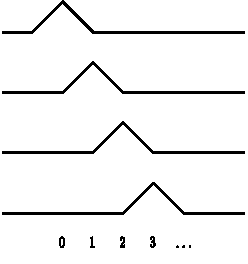
\includegraphics[width=0.5\linewidth]{img/pdf_compression/hist-kernels.pdf}
  \caption[Kernel functions]{%
    Visualization of triangular kernel functions for estimating the discrete probability mass histogram.%
  }
  \label{fig:pdf/kernels}
\end{figure}




\subsection{Loss function}
\label{sec:pdf_compression/loss}

Our model follows the variational formulation based on~\cite{balle2018variational}; further details on the construction may be found in earlier works such as~\cite{kingma2013autoencoding,balle2017endtoend,theis2017lossy}.
Briefly, for a variable $\boldvar{y}$, its counterparts $\tilde{\boldvar{y}}$ and $\hat{\boldvar{y}}$ denote the noise-modelled (for training) and quantized (for inference) versions of $\boldvar{y}$, respectively.
Furthermore, the variational encoder $q_{\boldvar{\phi}}(\boldvar{\tilde{y}}, \boldvar{\tilde{q}} \mid \boldvar{x})$ with trainable parameters $\phi$ is a probabilistic%
\footnote{During training, the encoder is probabilistic in order to model quantization via uniform noise.}
model of the joint distribution for $\boldvar{\tilde{y}}$ and $\boldvar{\tilde{q}}$, for a given input $\boldvar{x}$.
The loss function that we seek to minimize over the input data distribution $p_{\boldvar{x}}(\boldvar{x})$ can then be expressed as
%
\begin{equation*}
  \begin{split}
    \mathcal{L}
    &=
    \E_{\boldvar{x} \sim p_{\boldvar{x}}(\boldvar{x})}
    \E_{
      \boldvar{\tilde{y}}, \boldvar{\tilde{q}}
      \sim q_{\boldvar{\phi}}(\boldvar{\tilde{y}}, \boldvar{\tilde{q}} \mid \boldvar{x})
    }
    \left[
      -\log p_{\boldvar{\tilde{y}} \mid \boldvar{\tilde{q}}}(\boldvar{\tilde{y}} \mid \boldvar{\tilde{q}})
      - \lambda_q \log p_{\boldvar{\tilde{q}}}(\boldvar{\tilde{q}})
      + \lambda_x D(\boldvar{x}, \boldvar{\tilde{x}})
    \right]
    \\
    &=
    \E_{\boldvar{x} \sim p_{\boldvar{x}}(\boldvar{x})}
    \left[
      R_{\boldvar{\tilde{y}}}(\boldvar{x})
      + \lambda_q R_{\boldvar{\tilde{q}}}(\boldvar{x})
      + \lambda_x D(\boldvar{x}, \boldvar{\tilde{x}})
    \right].
  \end{split}
\end{equation*}
%
Here, $R_{\boldvar{\tilde{y}}}(\boldvar{x})$ and $R_{\boldvar{\tilde{q}}}(\boldvar{x})$ are the total rate costs of $\boldvar{\tilde{y}}$ and $\boldvar{\tilde{q}}$ for a given input $\boldvar{x}$, respectively.
Furthermore, $D(\boldvar{x}, \boldvar{\tilde{x}})$ is a distortion metric --- typically mean-squared error (MSE) --- between the input $\boldvar{x}$ and its reconstruction $\boldvar{\tilde{x}}$.
Additionally, $\lambda_x$ is a trade-off hyperparameter between the rate and distortion.
And lastly, $\lambda_q$ is a trade-off hyperparameter between the rate cost of encoding $\boldvar{\tilde{q}}$ against the amount of rate saved when using $\boldvar{\tilde{q}}$ to encode $\boldvar{\tilde{y}}$.

The choice for $\lambda_q$ depends upon the ratio between the target and trained-upon input dimensions:
\begin{equation*}
  \lambda_q =
  \frac%
  {H_{\boldvar{x}, \mathrm{trained}} W_{\boldvar{x}, \mathrm{trained}}}%
  {H_{\boldvar{x}, \mathrm{target}} W_{\boldvar{x}, \mathrm{target}}}.
\end{equation*}
For instance, for the target dimension of $768 \times 512$ (i.e., images from the Kodak test dataset) and a trained-upon dimension of $256 \times 256$ (i.e., image patches from the Vimeo-90K dataset), we set $\lambda_q = \frac{1}{6}$.

Let $\boldvar{p}_j = (p_{j1}, \ldots, p_{jB})$ refer to the discrete $B$-bin probability distribution
% (i.e., $0 \leq p_{ji} \leq 1$ and $\sum_i p_{ji} = 1$)
used to encode the $j$-th channel of $\boldvar{\tilde{y}}$.
Then concretely, the rate cost of $\boldvar{\tilde{y}}$ may be measured by the cross-entropy between the true and reconstructed%
\footnote{Since the reconstructed distribution is determined directly from $\boldvar{y}$ rather than from $\boldvar{\tilde{y}}$, we denote it by $\boldvar{\hat{p}}$, not $\boldvar{\tilde{p}}$.}
discretized distributions,
\begin{equation*}
  R_{\boldvar{\tilde{y}}}  % (\boldvar{x})
  % =
  % TODO {y, given x} notation is technically correct? Or is omitting it clearer?
  =
  \sum_{j=1}^{M}
  \sum_{i=1}^{B}  % \sum_{i=1}^{\operatorname{length}(\boldvar{\tilde{p}}_j)}
  -p_{ji} \log \hat{p}_{ji}.
\end{equation*}
Similarly, let $\boldvar{\tilde{q}}_j$ denote the $j$-th channel of $\boldvar{\tilde{q}}$.
Then, the rate cost of $\boldvar{\tilde{q}}$ is measured by the typical calculation,
\begin{equation*}
  R_{\boldvar{\tilde{q}}}  % (\boldvar{x})
  =
  \sum_{j=1}^{M}
  \sum_{i=1}^{\operatorname{length}(\boldvar{l}_j)}
  -{l_{ji}} \log {l_{ji}},
  \quad \text{where } {\boldvar{l}_j} = p_{\boldvar{\tilde{q}}_j}(\boldvar{\tilde{q}}_j).
\end{equation*}


% ORIGINAL FORMULATION, which may be interesting, but the new way is good enough...
%
%
% We define the rate of the compressed latent representation $\boldvar{\hat{\theta}}$ as
% $R_{\boldvar{\hat{\theta}}} = -\log \boldvar{\hat{p}}_{\boldvar{\hat{\theta}}}(\boldvar{\hat{\theta}})$.
% The "distortion" is defined as KL divergence between the true and reconstructed distributions, $D_{\mathrm{KL}}(\boldvar{p} \parallel \boldvar{\hat{p}})$.
% Let $\lambda$ be a trade-off parameter between rate and distortion.
% Then, the overall rate-distortion loss function is:
%
% \begin{equation*}
%   \mathcal{L}
%   = R_{\boldvar{\hat{\theta}}}
%   + \lambda \cdot D_{\mathrm{KL}}(\boldvar{p} \parallel \boldvar{\hat{p}})
% \end{equation*}
%
% The optimal choice for $\lambda$ is equal to the total number of latent pixels.
% For the Kodak dataset~\cite{kodak_dataset}, which contains $768 \times 512$ images, and a model with $16\times$ downscale factor, we set $\lambda = 48 \, \cdot \, 32 = 1536$.
% % To convert to bpp, it's $16 \cdot 16 = 256$.
%
% Due to the extra degree of freedom we obtain for probability distributions (i.e., probability distributions must sum to $1$ over their support), we may justifiably omit one symbol from the input.
% In particular, we choose to omit the "bypass" encoding mode symbol that represents symbols outside our finite support.
% This special symbol's probability value is sometimes referred to as the "tail mass".
% % To support such out-of-support symbols, the distortion term may be expanded as follows for a pseudo-distribution $\tilde{p}$
%
% We need to use an RD loss that accounts for the "missing" probability mass.
% r = (1 - pdf.sum()).clamp(min=0) pseudo-symbol.
%
% Due to the extra degree of freedom we obtain for probability distributions (i.e., probability distributions must sum to $1$ over their support), we may justifiably omit one symbol from the input.
% In particular, we choose to omit the "bypass" encoding mode symbol that represents symbols outside our finite support.
% This special symbol's probability value is sometimes referred to as the "tail mass".
% % To support such out-of-support symbols, the distortion term may be expanded as follows for a pseudo-distribution $\tilde{p}$, the loss becomes:




\subsection{Optimization}
\label{sec:pdf_compression/optimization}

We will now compute the derivatives for our proposed method.
To simplify the notation, within this subsection, we will focus on a single channel --- the $j$-th channel --- and directly denote $\boldvar{\tilde{y}}_j$ as $\boldvar{y}$, and $\boldvar{p}_j$ as $\boldvar{p}$.
Recall that from the perspective of the backward pass,
%
\begin{equation*}
  \begin{split}
    p_i
    &= (\operatorname{Histogram}(\boldvar{y}))_i \\
    &= \frac{1}{H W / s^2}
      \sum_n K_{\mathrm{soft}}{\left(\frac{y_n - b_i}{\Delta b}\right)} \\
    &= \frac{1}{H W / s^2}
      \sum_n \max \left\{ 0, 1 - \left| \frac{y_n - b_i}{\Delta b} \right| \right\},
  \end{split}
\end{equation*}
%
where $s$ is the downscale factor (e.g., $s = 2^4 = 16$ for a model with four downscaling strides of length $2$), and $H$ and $W$ are the height and width of the input image $\boldvar{x}$, respectively.
And so,
%
\begin{equation*}
  \begin{split}
    \frac{\partial p_i}{\partial y_k}
    &= \frac{1}{H W / s^2}
      \sum_n \frac{\partial}{\partial y_k} \left[
        \max \left\{ 0, 1 - \left| \frac{y_n - b_i}{\Delta b} \right| \right\}
      \right] \\
    &= \frac{1}{H W / s^2}
      \frac{\partial}{\partial y_k} \left[
        \max \left\{ 0, 1 - \left| \frac{y_k - b_i}{\Delta b} \right| \right\}
      \right] \\
    &= \frac{1}{H W / s^2} \cdot
      \frac{-1}{\Delta b} \cdot
      \underbrace{%
        H{\left( 1 - \left| \frac{y_k - b_i}{\Delta b} \right| \right)}
      }_{1 \text{ if } |y_k - b_i| < \Delta b \text{ else } 0}
      \cdot
      \underbrace{%
        \left( 2 \cdot H{\left( \frac{y_k - b_i}{\Delta b} \right)} - 1 \right)
      }_{-1 \text{ if } y_k < b_i \text{ else } 1},
  \end{split}
\end{equation*}
%
since
%
\begin{equation*}
  \frac{\partial}{\partial u} \max \{ 0, 1 - |u| \}
  = - H(1 - |u|) \cdot [2 \cdot H(u) - 1].
\end{equation*}
%
The corresponding derivative for the reconstructed distribution $\boldvar{\hat{p}}$ may be determined as
%
\begin{equation*}
  \begin{split}
    \frac{\partial \hat{p}_i}{\partial y_k}
    &= \sum_l
      \frac{\partial \hat{p}_i}{\partial p_l}
      \frac{\partial p_l}{\partial y_k}
    \\
    &\approx \sum_l
      \delta_{il}
      \frac{\partial p_l}{\partial y_k}
      \quad \text{assuming } \frac{\partial \hat{p}_i}{\partial p_l} \approx \delta_{il}
    \\
    &= \frac{\partial p_i}{\partial y_k},
  \end{split}
\end{equation*}
where we have assumed that the dominant term in the sum is the term where $l = i$.
% where $\delta_{il}$ is the Kronecker delta.

The rate cost of encoding the channel $\boldvar{y}$ with its associated discrete probability distribution $\boldvar{p}$ is given by
%
\begin{equation*}
  R_y = \frac{H W}{s^2} \sum_i -p_i \log \hat{p}_i.
\end{equation*}
%
Then, we may compute the derivative as follows:
%
\begin{equation}
  \label{eq:pdf_compression/optimization/dRdy_proposed}
  \begin{split}
    \frac{\partial R_y}{\partial y_k}
    &= \frac{-H W}{s^2} \sum_i \frac{\partial}{\partial y_k} \left[ p_i \log \hat{p}_i \right]
    \\
    &= \frac{-H W}{s^2} \sum_i \left[
      p_i \frac{\partial}{\partial y_k} \left[ \log \hat{p}_i \right]
      + \frac{\partial p_i}{\partial y_k} \log \hat{p}_i
    \right]
    \\
    &= \frac{-H W}{s^2} \sum_i \left[
      \frac{p_i}{\hat{p}_i} \frac{\partial \hat{p}_i}{\partial y_k}
      + \frac{\partial p_i}{\partial y_k} \log \hat{p}_i
    \right]
    \\
    &\approx \frac{-H W}{s^2} \sum_i \left[
      \frac{p_i}{\hat{p}_i} \frac{\partial p_i}{\partial y_k}
      + \frac{\partial p_i}{\partial y_k} \log \hat{p}_i
    \right]
    \quad \text{assuming } \frac{\partial \hat{p}_i}{\partial y_k} \approx \frac{\partial p_i}{\partial y_k}
    \\
    &= \frac{-H W}{s^2} \sum_i
      \left[ \frac{p_i}{\hat{p}_i} + \log \hat{p}_i \right]
      \frac{\partial p_i}{\partial y_k}
    \\
    &= \frac{-1}{\Delta b} \sum_i
      \left[ \frac{p_i}{\hat{p}_i} + \log \hat{p}_i \right] \cdot
      H{\left( 1 - \left| \frac{y_k - b_i}{\Delta b} \right| \right)} \cdot
      \left( 1 - 2 \cdot H{\left( \frac{y_k - b_i}{\Delta b} \right)} \right)
    \\
    &= \frac{-1}{\Delta b}
      \left(
        \left[ {\frac{p_i}{\hat{p}_i} + \log \hat{p}_i} \right]_{
          i=\lceil{y_k - y_{\mathrm{min}}}\rceil + 1
        }
        -
        \left[ {\frac{p_i}{\hat{p}_i} + \log \hat{p}_i} \right]_{
          i=\lfloor{y_k - y_{\mathrm{min}}}\rfloor + 1
        }
      \right)
    \\
    &\approx \frac{-1}{\Delta b} \left(
      \log \hat{p}_{\lceil{y_k - y_{\mathrm{min}}}\rceil + 1} -
      \log \hat{p}_{\lfloor{y_k - y_{\mathrm{min}}}\rfloor + 1}
    \right)
    \quad \text{assuming } \hat{p}_i \approx p_i.
  \end{split}
\end{equation}
%
Thus, assuming that $\hat{p}_i \approx p_i$ and $\frac{\partial \hat{p}_i}{\partial y_k} \approx \frac{\partial p_i}{\partial y_k}$, the gradient of the rate cost $R_y$ is directly proportional to the difference in code lengths of the two bins whose centers are nearest to the value $y_k$.
% Notably, the gradient is non-zero only for the two bins that contain the value $y_k$.
Intuitively, this makes sense, since the rate cost of encoding the $k$-th element is directly proportional to the linear interpolation between the code lengths of the two nearest bins:
%
\begin{equation*}
  R_{y_k} =
  -
  \left[
    \alpha \cdot
    \log \hat{p}_{\lfloor{y_k - y_{\mathrm{min}}}\rfloor + 1} +
    (1 - \alpha) \cdot
    \log \hat{p}_{\lceil{y_k - y_{\mathrm{min}}}\rceil + 1}
  \right],
\end{equation*}
%
where $\alpha
= (y_k - b_{\lfloor{y_k - y_{\mathrm{min}}}\rfloor + 1}) / \Delta b
= 1 - (b_{\lceil{y_k - y_{\mathrm{min}}}\rceil + 1} - y_k) / \Delta b$.
The linear interpolation may be justified by the fact that $\hat{y}_k$ inhabits only a single bin at a time.
The probability of $\hat{y}_k$ inhabiting the left bin is $\alpha$, and the probability of inhabiting the right bin is $1 - \alpha$.
This aligns perfectly with Shannon's measure of entropy, which is the expected value of the code length. % of a symbol.
(Isn't math elegant?)

% NOTE: p(y) is the "mass"; whereas, f(y) is the "density"

For comparison, the standard "entropy bottleneck" represents the likelihood of a symbol by
%
\begin{equation*}
  p(y)
  = c{\left(y + \frac{1}{2}\right)} - c{\left(y - \frac{1}{2}\right)}
  = \int_{y - \frac{1}{2}}^{y + \frac{1}{2}} f(t) \, dt,
\end{equation*}
%
where $c$ is the cumulative distribution function of the encoding distribution,
and $f(y) = \frac{d}{dy} c(y)$ is the probability density function of the encoding distribution.
Then, the rate cost for the "entropy bottleneck" is merely the sum of the negative log-likelihoods (i.e., code lengths),
%
\begin{equation*}
  R_y = \sum_i -\log p(y_i).
\end{equation*}
%
We may then compute its derivative as follows:
%
\begin{equation}
  \label{eq:pdf_compression/optimization/dRdy_standard}
  \begin{split}
    \frac{\partial R_y}{\partial y_k}
    &= - \sum_i \frac{\partial}{\partial y_k} \left[ \log p(y_i) \right] \\
    &= - \frac{\partial}{\partial y_k} \left[ \log p(y_k) \right] \\
    &= - \frac{1}{p(y_k)} \cdot \frac{\partial}{\partial y_k} \left[ p(y_k) \right] \\
    &= - \frac{1}{p(y_k)} \cdot \left[
      f{\left(y_k + \frac{1}{2}\right)} - f{\left(y_k - \frac{1}{2}\right)}
    \right].
  \end{split}
\end{equation}

Interestingly, whereas the derivative for the proposed method (under the assumption that $\hat{p}_i \approx p_i$) computed in \cref{eq:pdf_compression/optimization/dRdy_proposed} contains a difference between the "right" and "left" log-likelihoods,
the derivative for the standard method computed in \cref{eq:pdf_compression/optimization/dRdy_standard} contains a difference between the "right" and "left" evaluations of the probability density function.

% TODO(writing): criticize locality, or how if p is not p_hat, then gradient may be weird...
% Maybe do that elsewhere
% But is the locality the problem, or the log?!
% Or is it just the model design: f(y) parameterization is globally influenced at once, but p_i is not.

% TODO(experiment): I wonder if we could "replace" the derivatives so that the network trains?
% TODO(experiment): Maybe the problem is related to "sample rate"? The discrete bottleneck benefits from a higher sample rate of 4.




% \section{Discrete entropy bottleneck}
% \label{sec:pdf_compression/discrete_entropy_bottleneck}

% Does this need to be discussed? We didn't really use it.
% The sample rate trick is still interesting, though, as is the effects on training time.
% Actually, does it really take longer, since when we tried the default Balle factorized model with lambda=0.0067, that's also in 180+ epochs and counting... WHAT.
% And didn't we try discrete_entropy_bottleneck with same lambda, or was it lower?

% Essentially a "piecewise linear" entropy bottleneck
% Finite difference derivative smoothing kernel, etc.
% Sample rate. 1, 2, 4.
% Effects on training stability, etc.
% Seems to take longer to converge than the continuous cumulative logits formulation. (Why?)
% Compare training time
% Discrete indexing function.
% Computational graph showing d/df, and d/dx.

% TODO(figure): Training curves for DiscreteEntropyBottleneck




% \subsection{RDOQ}
%
% First, latent tune.
% Then, latent tune with (un)relaxation of discrete quantization step function.  (WOW, IDEA.)
% Then, random parallel greedy RDOQ with $\{-1, 0, +1\}$.
% And maybe heuristics (e.g. loss doesn't change for the channel on multiple passes, or the dLoss is low).
% Semi-random (i.e., every pixel is iterated over, i.e., 48*32 = 1536 pixels / channel)

% "Uninformed" RDOQ.




\section{Experimental setup}
\label{sec:pdf_compression/experimental_setup}

\subsection{Architecture details}
\label{sec:pdf_compression/experimental_setup/architecture_details}

As shown in \cref{fig:pdf/arch-hasq}, our $h_{a,q}$ and $h_{s,q}$ are implemented using a simple five-layer convolutional neural network.
In between each of the convolutional layers shown is a ReLU activation function, as well as a channel shuffle operation, as is done in ShuffleNet~\cite{zhang2017shufflenet}.
There are two strides of length $2$, resulting in a total downscaling factor of $s_q = 4$.
For all our models, we set $K = 15$ to control the kernel sizes, and $G = 8$ to control the number of channel groups.
Furthermore, we set $(N_q, M_q) = (32, 16)$ for low-resolution models, and $(N_q, M_q) = (64, 32)$ for high-resolution models.
The number of bins $B$ is set between $128$ and $1024$ across different models.
We have elected to use an entropy bottleneck design for simplicity, though one can likely further improve the compression performance of the probability distribution compression architecture by using more powerful entropy modeling techniques (e.g., a scale hyperprior).
% TODO(review): Move this to "future work"?
Since $\lambda_q$ is a parameter that depends on the ratio between the target and trained-upon input dimensions, it may also be advisable to train a single model which that supports $\lambda$-rate control strategies (e.g., G-VAE~\cite{cui2020gvae,cui2022asymmetric} and QVRF~\cite{tong2023qvrf}) for both latent representations $y, q$.
However, we have not yet explored this possibility.
% NOTE: I suppose this can be a "discussion" explaining why model may work:
%
% One may even consider replacing the convolutions with linear basis functions such as Gaussians.
% However, convolutions with sufficiently large kernel windows already encompass the class of functions approximated by finitely-supported basis functions.%
% \footnote{%
%   To quote Geoffrey Hinton from his talk~\cite{hinton2017capsulestalk}, "the fact that [CNNs] work so well is extremely unfortunate".%
%   % https://www.youtube.com/watch?v=rTawFwUvnLE&t=510s
% }

\begin{figure}[htbp]
  \centering
  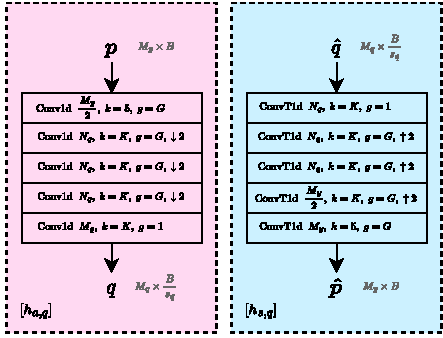
\includegraphics[width=1.0\linewidth]{img/pdf_compression/arch-hasq.pdf}
  \caption[Architecture layer diagram for $h_{a,q}$ and $h_{s,q}$ transforms]{%
    Architecture layer diagram for $h_{a,q}$ and $h_{s,q}$ transforms.
    $k$ denotes kernel size, $g$ denotes number of channel groups, and $\downarrow, \uparrow$ denote stride.%
  }
  \label{fig:pdf/arch-hasq}
\end{figure}




\subsection{Training details}
\label{sec:pdf_compression/experimental_setup/training_details}

% Pretty standard setup for batch size, optimizer, LR scheduler, dataset, etc:
Our models are trained on $256 \times 256$ image patches from the Vimeo-90K triplet dataset~\cite{xue2019video}.
A training batch size of $16$ was used, along with the Adam optimizer~\cite{kingma2014adam} with an initial learning rate of $10^{-4}$ that was decayed by a factor of $0.1$ whenever the validation loss plateaued.
Specifically, we loaded the weights of the pretrained models from CompressAI~\cite{begaint2020compressai}, which were also trained using the same setup as above.
We replaced the static distributions of the EntropyBottleneck module with the dynamically generated adaptive distributions from our proposed probability distribution compression module.
Then, we froze the weights for $g_a$ and $g_s$, and trained only the weights for our probability distribution compression model (i.e., for $h_{a,q}$ and $h_{s,q}$, and the entropy model for $q$).
Finally, we evaluated our models on the standard Kodak test dataset~\cite{kodak_dataset} containing 24 images of size $768 \times 512$.
(Thus, we set $\lambda_q = \frac{1}{6}$ during training.)




\section{Experimental results}
\label{sec:pdf_compression/experimental_results}

\cref{fig:pdf/rd-curves} shows the rate-distortion (RD) curves comparing a given base model against the same model enhanced with our proposed probability distribution compression module.


\begin{figure}[htbp]
  \centering
  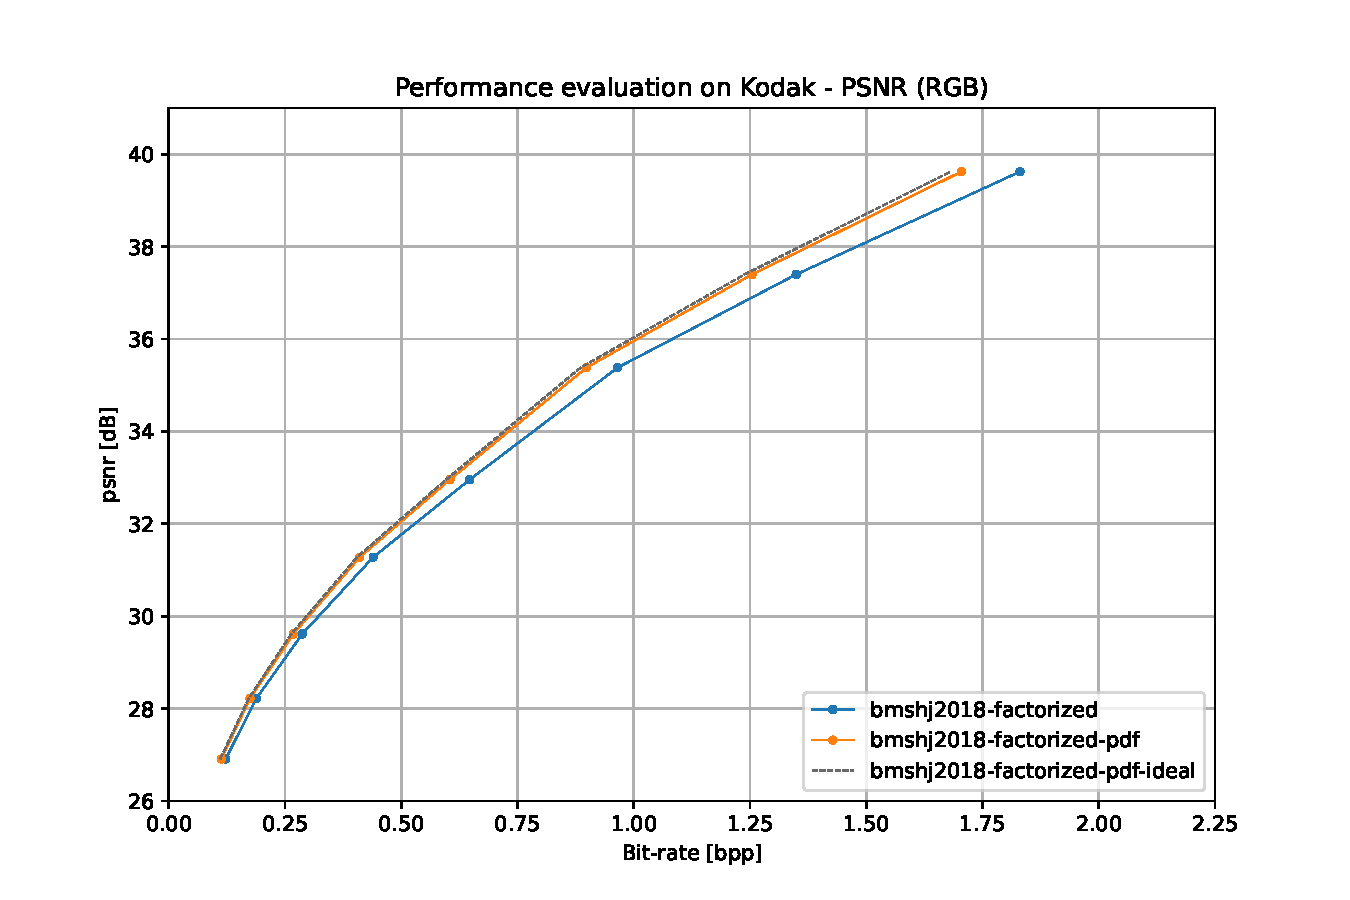
\includegraphics[width=\linewidth]{img/pdf_compression/rd-curves-kodak-psnr-bmshj2018-factorized.pdf}
  \caption[RD curves for Kodak dataset]{%
    RD curves for the Kodak dataset.%
  }
  \label{fig:pdf/rd-curves}
\end{figure}


In~\cref{tbl:pdf}, we compare the rate savings of our proposed method against the base model at various quality levels.
Additionally, we also list the maximum rate savings that can be theoretically achieved by perfectly eliminating the amortization gap between the true and reconstructed distributions, i.e., by using the true distribution directly as the encoding distribution with zero additional transmission cost.
As shown, our approach achieves a 6.95\% BD-rate reduction over the base model, in comparison to a maximum possible reduction of 8.33\% BD-rate reduction achievable by perfectly eliminating the amortization gap.


% Q  Rate savings (per latent pixel)
% 1    2.922
% 2    4.116
% 3    5.941
% 4    8.827
% 5   12.866
% 6   20.265
% 7   28.392
% 8   37.989
%
% For 16x downscale (e.g. 768x512 input -> 48x32 latent), the maximum potential rate saved per image pixel is:
% >>> np.array([2.922, 4.116, 5.941, 8.827, 12.866, 20.265, 28.392, 37.989]) / (16 * 16)
% array([0.011, 0.016, 0.023, 0.034, 0.050, 0.079, 0.111, 0.148])


% TODO Maybe measure base model bpp as bpp_loss.
\begin{table}[htbp]
  \centering
  \caption[Rate savings for the bmshj2018-factorized model at various qualities]{%
    Potential and achieved rate savings for the bmshj2018-factorized model~\cite{balle2018variational} when equipped with our proposed distribution compression method.%
  }
  \label{tbl:pdf}
  \small
  \begin{tabular}[]{ccccccc}
    \toprule
    % TODO(review): Reorder columns for easier comparison?
    \thead{Quality}
    & \thead{Original \\ (bpp)}
    & \thead{Potential \\ gain (bpp)}
    & \thead{Potential \\ BD-rate}
    & \thead{Our \\ (bpp)}
    & \thead{Our gain \\ (bpp)}
    & \thead{Our \\ BD-rate} \\
    \midrule
    1 & 0.122 & -0.012 & -9.45 & 0.113 & -0.009 & -7.66 \\
    2 & 0.188 & -0.016 & -8.66 & 0.175 & -0.013 & -7.13 \\
    3 & 0.287 & -0.024 & -8.20 & 0.268 & -0.019 & -6.76 \\
    4 & 0.440 & -0.035 & -7.90 & 0.411 & -0.029 & -6.57 \\
    5 & 0.647 & -0.051 & -7.83 & 0.605 & -0.043 & -6.57 \\
    6 & 0.965 & -0.080 & -8.25 & 0.898 & -0.067 & -6.95 \\
    7 & 1.349 & -0.111 & -8.24 & 1.254 & -0.095 & -7.04 \\
    8 & 1.830 & -0.149 & -8.14 & 1.705 & -0.126 & -6.88 \\
    mean &    &        & -8.33 &       &        & -6.95 \\
    \bottomrule
  \end{tabular}
\end{table}


In order to compute the potential savings, we first ran the base model on each image from the Kodak test dataset~\cite{kodak_dataset}, giving us a collection of true distributions $\boldvar{p}$ for each image.
Furthermore, the base model provides a static encoding distribution $\boldvar{p_{\textnormal{default}}}$.
% TODO(review): Move formula to earlier section, then reference here?
Then, we computed the potential savings (in bpp) for each image as
$(\Delta R)_{\textnormal{max}} = \frac{HW / s^2}{HW} \sum_j D_{\mathrm{KL}}(\boldvar{p}_j \parallel (\boldvar{p_{\textnormal{default}}})_j)$.
We then averaged these values across the entire dataset.



% TODO(review): Mention the following tables within the main body text.

\begin{table}[htbp]
  \centering
  \caption{%
    Comparison of rates for various models.
    Ratio is the fraction of the total rate occupied original unmodified model.
    % TODO(review): Contrary to balcilar2022amortizationgap, it might be more natural to report in "absolute" percentage of total bitstream, rather than percentage of the given latent bitstream? (i.e., multiply)
    % TODO(review): Maybe Potential, Actual are better names than Gap, Gain?
    Gap is the maximum potential savings with perfect distribution reconstruction and zero additional transmission cost.
    Gain is the actual change in rate achieved by the given method.
    All results are reported for the Kodak dataset~\cite{kodak_dataset}.%
  }
  \label{tbl:rate-gains}
  \small
  \begin{tabular}[]{ccccc}
    \toprule
    \multirow{4}{*}{\thead{Model}}
    & \multicolumn{3}{c}{\thead{Factorized}}
    & \multicolumn{1}{c}{\thead{Total}}
    \\
    \cmidrule(lr){2-4}
    \cmidrule(lr){5-5}
    & \thead{Ratio \\ (\%)}
    & \thead{Gap   \\ (\%)}
    & \thead{Gain  \\ (\%)}
    & \thead{Gain  \\ (\%)}
    \\
    \midrule
    bmshj2018-factorized~\cite{balle2018variational} + \cite{balcilar2022amortizationgap} (Q=1)
      &   100 & -9.45 & -6.79 & -6.79 \\
    bmshj2018-factorized~\cite{balle2018variational} + ours (Q=1)
      &   100 & -9.45 & -7.66 & -7.66  \\
    % TODO digitize and measure:
    % bmshj2018-factorized~\cite{balle2018variational} + \cite{balcilar2022amortizationgap}
    %   &   100 & -... & -... & -... \\  % TODO
    bmshj2018-factorized~\cite{balle2018variational} + ours
      &   100 & -8.33 & -6.95 & -6.95  \\
    % TODO
    % mbt2018-mean~\cite{minnen2018joint} + \cite{balcilar2022amortizationgap}
    % mbt2018-mean~\cite{minnen2018joint} + ours
    \bottomrule
  \end{tabular}
\end{table}


\begin{table}[htbp]
  \centering
  \caption{%
    Trainable parameter counts and number of multiply-accumulate operations (MACs) per pixel.
    All results are reported for the Kodak dataset~\cite{kodak_dataset}.%
  }
  \label{tbl:pdf/params-macs}
  \small
  \begin{tabular}[]{ccccc}
    \toprule
    % TODO(review): Make the table more horizontally compact?
    % \multirow{3}{*}[1ex]{\thead{Model \\ configuration \\[3pt] $(N_q, M_q, K, G, B)$}}
    \thead{Model configuration}
    & \thead{Params}
    & \thead{MACs/pixel}
    & \thead{Params}
    & \thead{MACs/pixel}
    \\
    \midrule
    \thead{$(M_y, N_q, M_q, K, G, B)$}
    & \multicolumn{2}{c}{\thead{$h_{a,q}$}}
    & \multicolumn{2}{c}{\thead{$h_{s,q}$}}
    \\
    \cmidrule(lr){1-1}
    \cmidrule(lr){2-3}
    \cmidrule(lr){4-5}
    %
    % def params(in_channels, out_channels, kernel_size, groups, stride_total, dim):
    %     return in_channels * out_channels * kernel_size**dim / groups
    %
    % def macs(in_channels, out_channels, kernel_size, groups, stride_total, dim):
    %     return (
    %         in_channels * out_channels * kernel_size**dim / groups / stride_total**dim
    %     )
    %
    % def compute(M_y, N_q, M_q, K, G, B, dim):
    %     fs = {"params": params, "macs": macs}
    %     results = {}
    %     for key, f in fs.items():
    %         results[key] = sum(
    %             [
    %                 f(M_y, M_y // 2, 5, G, 1, dim),
    %                 f(M_y // 2, N_q, K, G, 2, dim),
    %                 f(N_q, N_q, K, G, 4, dim),
    %                 f(N_q, N_q, K, G, 8, dim),
    %                 f(N_q, M_q, K, 1, 8, dim),
    %             ]
    %         ) * (B / (768 * 512) if key == "macs" else 1)
    %     return results
    %
    % print(compute(M_y=192, N_q=32, M_q=16, K=15, G=8, B=256, dim=1))
    % print(compute(M_y=320, N_q=64, M_q=32, K=15, G=8, B=1024, dim=1))
    %
    Ours $(192, 32, 16, 15, 8, 256)$  & 0.029M & 10 & 0.029M & 10 \\
    Ours $(320, 64, 32, 15, 8, 1024)$ & 0.097M & 126 & 0.097M & 126 \\[3pt]
    \midrule
    \thead{$(N, M)$}
    & \multicolumn{2}{c}{\thead{$h_{a}$}}
    & \multicolumn{2}{c}{\thead{$h_{s}$}}
    \\
    \cmidrule(lr){1-1}
    \cmidrule(lr){2-3}
    \cmidrule(lr){4-5}
    bmshj2018-hyperprior~\cite{balle2018variational} $(128, 192)$ & 1.040M & 1364 & 1.040M & 1364 \\
    bmshj2018-hyperprior~\cite{balle2018variational} $(192, 320)$ & 2.396M & 3285 & 2.396M & 3285 \\[3pt]
    \bottomrule
  \end{tabular}
\end{table}


% TODO(table): Cost of distribution transmission (e.g. 0.0002 bpp or ___ bits or ___% of bitstream, for Kodak)?


% TODO(writing): Mention how unfreezing g_a, g_s, and entropy_bottleneck results in poorer performance than keeping them frozen.


% TODO(experiment):
%
% PDF+RDOQ
%
% Factorized relu: mini, lite, original
% Factorized: mini, lite, original
% ELIC, cheng, mbt-mean, hyperprior

\FloatBarrier




\section{Conclusion}
\label{sec:pdf_compression/conclusion}

In this chapter, we proposed a learned method for the compression of probability distributions.
Our method effectively measures and compresses the encoding distributions used by the entropy bottleneck.
The experiments we performed where we only trained the distribution compression component show that this method is effective at significantly reducing the amortization gap.
Since many learned compression models use the entropy bottleneck component, our method provides them with a low-cost potential improvement in bitrate.
Furthermore, our work opens up the possibility of using learned distribution compression as a paradigm for correcting encoding distributions.

% Our results demonstrate that our method can significantly reduce the effect of the amortization gap, thereby achieving nearly the full breadth of theoretically possible gains for the pretrained base models with frozen transform parameters.
% Thus, the entropy bottleneck becomes adaptive.


% TODO(discussion):
%
% Possible reasons end-to-end doesn't work well:
%
% - Mean/median drift (e.g. part of y distribution goes outside the support)
%   Maybe add an assert to check if histogram(y).sum() == H * W;
%   or that the OOB (1 - p.sum()) < 0.01.
% - Number of bins insufficient.
% - OOB needs to be in loss function.
% - Derivatives are too "local". And don't really capture global behavior, especially once the distribution becomes bimodal.
%
% What I am doing to remedy this:
%
% - Compare derivatives...
% - Ensure g_a receives derivatives, of similar magnitude or average direction. Maybe just compare first few iterations...
% - Consider "CDF logits" style implementation, which was more successful in the past.




\subsection{Future work}
\label{sec:pdf_compression/conclusion/future_work}

A few steps remain towards making probability distribution corrective methods viable parts of more advanced entropy models such as~\cite{balle2018variational,cheng2020learned,he2022elic}.
These include the following:
%
% TODO(writing): trim; reword
\begin{itemize}
  \item
    The proposed adaptive entropy bottleneck needs to be formulated in such a way that it can be trained fully end-to-end.
    When training a pretrained base model equipped with our adaptive distribution compression module, we found that unfreezing the pretrained transform weights led to a degradation in RD performance.
    In contrast, keeping the transform frozen led to improvements in RD performance.
    This suggests that the rate-minimizing gradients flowing backwards into the transform through our adaptive distribution compression module are not necessarily well-formulated.
  \item
    Application of our adaptive distribution method to the Gaussian conditional component of entropy models.
    This component (along with the entropy bottleneck) is used to construct entropy modeling methods such as those used in~\cite{balle2018variational,cheng2020learned,he2022elic}.
    Most SOTA learned image compression models predict the parameters of the Gaussian or Gaussian mixture encoding distributions using various sophisticated methods.
    However, in all such models, the focus has been on optimizing the location and scale of the fixed Gaussian-shaped distributions.
    Thus, there are potential rate improvements to be made by adapting the shapes of the encoding distributions to shapes that more closely match the data distribution.
    (One such effort is Gaussian-Laplacian-Logistic Mixture Model (GLLMM) proposed in~\cite{fu2021learned}.)
    One way to directly apply our adaptive distribution method to Gaussian distributions would be to discretize them and then run the result through a distribution compression model.
    % Obviously, using Conv3d is the natural choice for this, where $\boldvar{p}$ $\hat{\boldvar{p}}$ has the shape $M \times H \times W \times B$.
    % We can also concatenate with $y$ embedded as delta distributions, i.e., a shape of $M \times H \times W \times B$.
    %
    % Our adaptive method for correcting the encoding distribution is currently only applied to the entropy bottleneck.
    % Such as discretization.
\end{itemize}




% TODO(writing):  [Maybe in another chapter]
% - I have also improved the RDOQ process introduced in "Entropy Coding Improvement for Low-complexity Compressive Auto-encoders" with a parallelized version that gives better results.

% TODO(experiment):
%
%
% RDOQ:
%
% Pre-tune via ~\cite{campos2019content}
% Serial is slow, and has less ... and more "bias"...
% Parallel with sufficient distance, or prone to divergence.
% We chose +/-9 (I think? or radius=4?) latent region of influence (or whatever it's called)
% Noise helps with "bias" ...
% Use noise to choose initially, then focus on the ones that change the most.
%
% Improve RDOQ with half the latent window or something like that?
% Or even multiple channels optimized at once...
% Divergence/convergence controller with backtracking.
%
% Why not allow RDOQ drifting from plus minus 1 based on its present state rather than a fixed origin?
% Maybe latent tune then random parallel RDOQ. Fast!? And heuristics, greedy?
% Maybe latent tune and slowly unrelax the quantization model to a discrete step activation function. (WOW, IDEA.)
%
%
%
% MISC:
%
% Also, I wonder if there is a "regularizer" or optimizer or reparameterization that helps prevent entropy models from getting stuck in "clusters" of probability... And helps them merge/split probabilities as needed.
% Perhaps a "coarse-to-fine" c(x) function, or one with clever normalizing flows, rather than matrix multiply 3 nodes with 4 layers or whatever.
%
% Might be interesting to post train various entropy models on top of factorized...
% I wonder which would be best.
% Or if we could make it simpler once the transform is fixed.
% Also eliminates bidirectional effects where the data itself contains way more redundancy than it would under the fully factorized assumption.




% TODO(writing): Define abbreviations. bpp, BD, RD, KL, etc.
% TODO(writing): Consistency: R_y, or R_{\boldvar{\tilde{y}}}? Same for R_q.

% TODO(figure): [SUPER-EASY] MS-SSIM (dB) RD curves; measure average of per-sample MS-SSIM dB.
% TODO(figure): [SUPER-EASY] RD curves for MS-SSIM, CLIC-2021 professional test dataset.
% TODO(figure): [EASY] (just subtract the base and write to another JSON) RD curves flattened w.r.t. base, like balcilar2022amortizationgap.
% TODO(figure): [EASY.]  Entropy bottleneck distributions (e.g. from plotly).
% TODO(figure): [EASY.]  Per-channel rate histograms.
% TODO(figure): Explain Entropy bottleneck, Gaussian conditional, etc. For introduction.
% TODO(figure): Initial vs final distributions plotly (or mpl) as PDF
